\chapter{Design}
	
	In this chapter a system design is proposed based on the considerations of the
	previous chapter. An overview is given which is followed by a more detailed
	description of the important components of the system.
	
	\section{Overview}
		
		The 3D Printing system can be divided up into three main parts. First is the
		computer software used to design the object to be printed and to generate
		the G-code instructions which will cause the object to be printed. The
		second is microcontroller firmware which processes the G-code and drives the
		printer electronics appropriately. Finally, there are the actual printer
		hardware consisting of electronics driving the various motors, heaters and
		sensors.
		
		Figure \ref{fig:systemDiagramTop} shows how the three main parts are broken
		down and each component will be described in detail in the following
		sections. This project focuses on the firmware and hardware with design and
		G-code production left to standard tools such as ReplicatorG and Skeinforge.
		
		\begin{figure}
			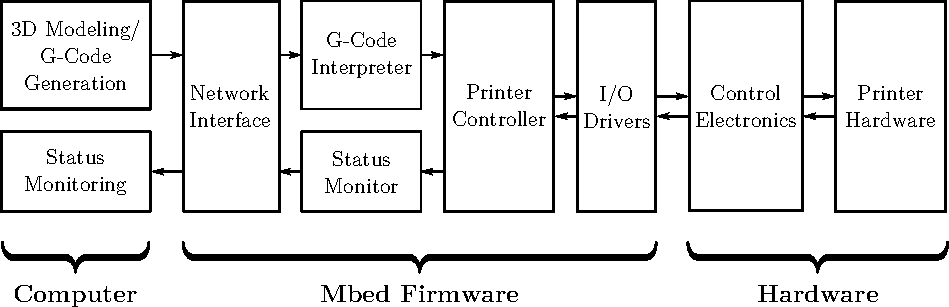
\includegraphics[width=1\textwidth]{diagrams/systemDiagramTop.pdf}
			% TODO: Explain what greyed out boxes mean.
			\caption{High-level diagram of overall system architecture.}
			\label{fig:systemDiagramTop}
		\end{figure}
	
	\section{Firmware}
		
		The firmware will be built on top of FreeRTOS which will allow easy
		separation of the various components of the firmware and facilitate
		communication between them.
		
		\subsection{G-Code Processing}
			
			\begin{figure}[here]
				
\includegraphics[width=1\textwidth]{diagrams/firmwarePipeline.pdf}
				\caption{The firmware G-code processing pipeline}
				\label{fig:firmwarePipeline}
			\end{figure}
	
	\section{Hardware}
		
		\subsection{Microcontroller}
		
		\subsection{Stepper Control}
		
		\subsection{Heater \& DC Motor Control}
	
